\begin{frame}{\textbf{Motivations}}

\begin{itemize}
\item Growing number of publications and conferences
\item To read through all documents is impossible
\item To search for poster is very difficult. See SfN search website \href{http://www.abstractsonline.com/plan/BrowseResults.aspx?date=11/15/2014&mkey=\%7B54C85D94-6D69-4B09-AFAA-502C0E680CA7\%7D}{\textcolor{gray}{here}}.
\item It's a large-scale problem that requires real-time answers
\item Ability to search new documents, relevant documents and group of people who work on the same problem
\end{itemize}

\end{frame}


\begin{frame}{\textbf{Proposal}}

\begin{itemize}
\item People are good at telling when they like or dislike something
\item We need automated analysis of content because topics change quickly, especially at conferences
\item We need the community to try and test different approaches to solve this problem - reproducibility through open-source
\end{itemize}

\end{frame}


\begin{frame}{\textbf{Scholarfy: application}}

\begin{figure}
\href{http://www.scholarfy.net}{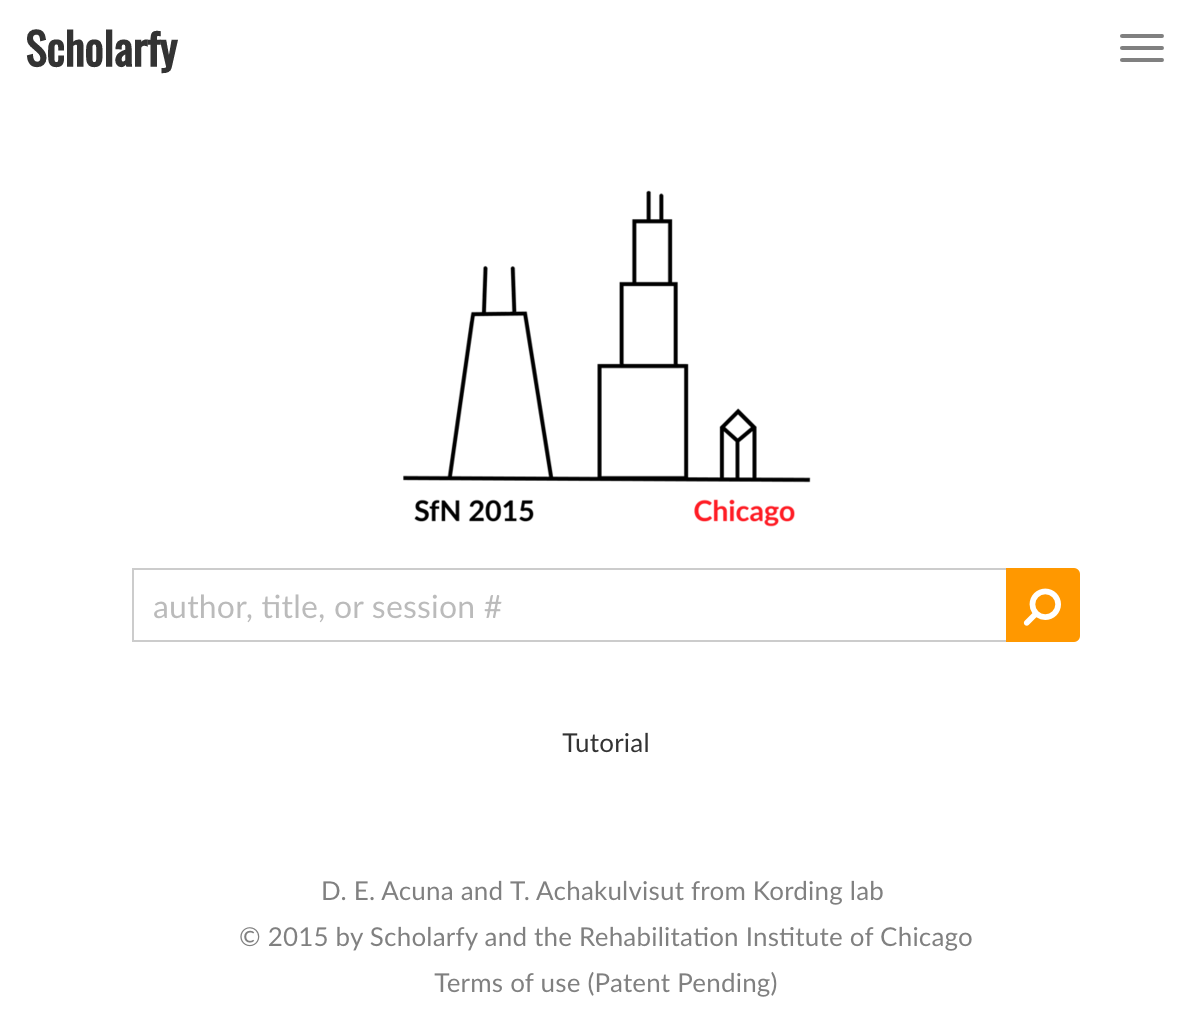
\includegraphics[width=2.5in]{images/scholarfy}}\\
\end{figure}

7500 sessions, 2900 users, \\
48000 page views, 6 minutes average per session

\end{frame}


\begin{frame}{\textbf{Data and Problems}}

\begin{itemize}

\item Data
\begin{itemize}
\item Scrape data from SfN \href{http://www.abstractsonline.com/plan/BrowseResults.aspx?date=11/15/2014&mkey=\%7B54C85D94-6D69-4B09-AFAA-502C0E680CA7\%7D}{\textcolor{gray}{website}} (with permission)
\item 15k posters, 70k total authors, 53k unique authors
\end{itemize}


\item The solution has 2 main parts:
\begin{itemize}
\item \textbf{Abstract representation} \textit{i.e. how to represent abstract in vector space?}
\item \textbf{Abstract recommendation} \textit{i.e. how to suggest posters to conference-goers}?
\end{itemize}

\end{itemize}

\end{frame}